\chapter{Additional information to Chapter~\ref{chapter:2024-sym-domains}}
\label{appendix:2024-sym-domains}

%%%%%%%%%%%%%%%%%%%%%%%%%%%%%%%%%%%%%%%%%%%%%%%%%%%%%%%%%%%%%%%%%%%%%%%%
%%%%%%%%%%%%%%%%%%%%%%%%%%%%%%%%%%%%%%%%%%%%%%%%%%%%%%%%%%%%%%%%%%%%%%%%
\section{Supplementary tables}


\begin{table}[h]
    \centering
    \caption[Basic descriptive characteristics of healthy controls and ME/CFS patients]{Basic descriptive characteristics of healthy controls and ME/CFS patients. Patients were considered to be a single population, two subgroups based on the severity of symptoms (mild to moderate or severely affected), or four subgroups according to the responses about infection triggers given in the symptoms' assessment questionnaire (S0, S1, S2, or S3). P-values refer to Pearson's Chi-squared test for qualitative measures and the two-sided Kruskal-Wallis rank sum test on the quantitative medians. HC, Healthy control; S0, Do not know; S1, Non-infection trigger; S2, Infection trigger but not confirmed with a lab test; S3, Infection trigger confirmed with a lab test; SD, Standard deviation; Min, Minimum; Max, Maximum.}
    \resizebox{\linewidth}{!}{% \begin{tabular}{lccccccccccccccc} 
% \toprule
% \multicolumn{1}{c}{} & \multirow{2}{*}{\begin{tabular}[c]{@{}c@{}}HC\\(n = 106)\end{tabular}} & \multirow{2}{*}{\begin{tabular}[c]{@{}c@{}}ME/CFS\\(n = 241)\end{tabular}} & \multirow{2}{*}{P-value} & & \multicolumn{4}{c}{Severity} & & \multicolumn{6}{c}{Infection trigger} \\ 
% \cmidrule{6-9}\cmidrule{11-16}
% \multicolumn{1}{c}{} & & & & & \begin{tabular}[c]{@{}c@{}}Mild/Moderate\\(n = 188)\end{tabular} & \begin{tabular}[c]{@{}c@{}}Severe\\(n = 53)\end{tabular} & \begin{tabular}[c]{@{}c@{}}P-value,\\ME/CFS only\end{tabular} & P-value & & \begin{tabular}[c]{@{}c@{}}S0\\(n = 61)\end{tabular} & \begin{tabular}[c]{@{}c@{}}S1\\(n = 43)\end{tabular} & \begin{tabular}[c]{@{}c@{}}S2\\(n = 91)\end{tabular} & \begin{tabular}[c]{@{}c@{}}S3\\(n = 47)\end{tabular} & P-value, ME/CFS only & P-value \\ 
% \cmidrule{2-16}
% Sex & & & 0.819 & & & & \textcolor{red}{1} & 0.922 & & & & & & 0.642 & 0.775 \\
% Female (\%) & 79 (74.5) & 184 (76.3) & & & 144 (76.6) & 40 (75.5) & & & & 46 (75.4) & 33 (76.7) & 72 (80.0) & 33 (70.2) & & \\
% Male (\%) & 27 (25.5) & 57 (23.7) & & & 44 (23.4) & 13 (24.5) & & & & 15 (24.6) & 10 (23.3) & 18 (20.0) & 14 (29.8) & & \\
% Age & & & 0.827 & & & & 0.799 & 0.947 & & & & & & 0.338 & 0.497 \\
% Mean (SD) & 41.7 (11.7) & 42.2 (11.0) & & & 42.0 (11.0) & 42.5 (11.1) & & & & 43.5 (10.2) & 40.2 (13.0) & 43.1 (10.8) & 40.5 (10.4) & & \\
% Median [Min, Max] & 43.0 [18.0, 60.0] & 43.0 [18.0, 60.0] & & & 43.0 [18.0, 60.0] & 46.0 [18.0, 59.0] & & & & 44.0 [22.0, 59.0] & 41.0 [18.0, 60.0] & 43.5 [18.0, 59.0] & 41.0 [18.0, 57.0] & & \\
% Disease duration & & & --- & & & & \textcolor{red}{0.001} & --- & & & & & & 0.495 & --- \\
% Mean (SD) & --- & 12.4 (8.3) & & & 11.4 (7.98) & 15.8 (8.58) & & & & 12.3 (7.79) & 11.6 (8.59) & 12.0 (8.57) & 13.7 (8.28) & & \\
% Median [Max, Min] & --- & 11.2 [0.2, 39.9] & & & 9.8 [0.2, 38.0] & 15.7 [1.5, 39.9] & & & & 11.1 [1.4, 37.0] & 9.5 [1.6, 38.0] & 11.0 [0.2, 39.9] & 12.9 [1.1, 29.3] & & \\
% Missing (\%) & 106 (100) & 5 (2.1) & & & 5 (2.7) & 0 (0.) & & & & 2 (3.3) & 2 (4.7) & 1 (1.1) & 0 (0.0) & & \\
% ME/CFS diagnosis & & & --- & & & & \textcolor{red}{0.004} & --- & & & & & & 0.095 & --- \\
% 1994 CDC only (\%) & --- & 33 (13.7) & & & 33 (17.6) & 0 (0.0) & & & & 12 (19.7) & 10 (23.3) & 6 (6.7) & 5 (10.6) & & \\
% 2003 CCC only (\%) & --- & 3 (1.2) & & & 2 (1.1) & 1 (1.9) & & & & 0 (0.0) & 1 (2.3) & 1 (1.1) & 1 (2.1) & & \\
% 1994 CDC/2003 CCC (\%) & --- & 205 (85.1) & & & 153 (81.4) & 52 (98.1) & & & & 49 (80.3) & 32 (74.4) & 83 (92.2) & 41 (87.2) & & \\
% \bottomrule
% \end{tabular}

\begin{tabular}{lccccccccccccccc} 
\toprule
\multicolumn{1}{c}{} & \multirow{2}{*}{\begin{tabular}[c]{@{}c@{}}HC\\(n = 106)\end{tabular}} & \multirow{2}{*}{\begin{tabular}[c]{@{}c@{}}ME/CFS\\(n = 241)\end{tabular}} & \multirow{2}{*}{P-value} & & \multicolumn{4}{c}{Severity} & & \multicolumn{6}{c}{Infection trigger} \\ 
\cmidrule{6-9}\cmidrule{11-16}
\multicolumn{1}{c}{} & & & & & \begin{tabular}[c]{@{}c@{}}Mild/Moderate\\(n = 188)\end{tabular} & \begin{tabular}[c]{@{}c@{}}Severe\\(n = 53)\end{tabular} & \begin{tabular}[c]{@{}c@{}}P-value,\\ME/CFS only\end{tabular} & P-value & & \begin{tabular}[c]{@{}c@{}}S0\\(n = 61)\end{tabular} & \begin{tabular}[c]{@{}c@{}}S1\\(n = 43)\end{tabular} & \begin{tabular}[c]{@{}c@{}}S2\\(n = 91)\end{tabular} & \begin{tabular}[c]{@{}c@{}}S3\\(n = 47)\end{tabular} & P-value, ME/CFS only & P-value \\ 
\cmidrule{1-16}
Sex & & & 0.819 & & & & $\approx$1.000 & 0.922 & & & & & & 0.642 & 0.775 \\
~~~Female (\%) & 79 (74.5) & 184 (76.3) & & & 144 (76.6) & 40 (75.5) & & & & 46 (75.4) & 33 (76.7) & 72 (80.0) & 33 (70.2) & & \\
~~~Male (\%) & 27 (25.5) & 57 (23.7) & & & 44 (23.4) & 13 (24.5) & & & & 15 (24.6) & 10 (23.3) & 18 (20.0) & 14 (29.8) & & \\
&&&&&&&&&&&&&&& \\
Age & & & 0.827 & & & & 0.799 & 0.947 & & & & & & 0.338 & 0.497 \\
~~~Mean (SD) & 41.7 (11.7) & 42.2 (11.0) & & & 42.0 (11.0) & 42.5 (11.1) & & & & 43.5 (10.2) & 40.2 (13.0) & 43.1 (10.8) & 40.5 (10.4) & & \\
~~~Median [Min, Max] & 43.0 [18.0, 60.0] & 43.0 [18.0, 60.0] & & & 43.0 [18.0, 60.0] & 46.0 [18.0, 59.0] & & & & 44.0 [22.0, 59.0] & 41.0 [18.0, 60.0] & 43.5 [18.0, 59.0] & 41.0 [18.0, 57.0] & & \\
&&&&&&&&&&&&&&& \\
Disease duration & & & --- & & & & 0.001 & --- & & & & & & 0.495 & --- \\
~~~Mean (SD) & --- & 12.4 (8.3) & & & 11.4 (7.98) & 15.8 (8.58) & & & & 12.3 (7.79) & 11.6 (8.59) & 12.0 (8.57) & 13.7 (8.28) & & \\
~~~Median [Max, Min] & --- & 11.2 [0.2, 39.9] & & & 9.8 [0.2, 38.0] & 15.7 [1.5, 39.9] & & & & 11.1 [1.4, 37.0] & 9.5 [1.6, 38.0] & 11.0 [0.2, 39.9] & 12.9 [1.1, 29.3] & & \\
~~~Missing (\%) & 106 (100) & 5 (2.1) & & & 5 (2.7) & 0 (0.0) & & & & 2 (3.3) & 2 (4.7) & 1 (1.1) & 0 (0.0) & & \\
&&&&&&&&&&&&&&& \\
ME/CFS diagnosis & & & --- & & & & 0.004 & --- & & & & & & 0.095 & --- \\
~~~1994 CDC only (\%) & --- & 33 (13.7) & & & 33 (17.6) & 0 (0.0) & & & & 12 (19.7) & 10 (23.3) & 6 (6.7) & 5 (10.6) & & \\
~~~2003 CCC only (\%) & --- & 3 (1.2) & & & 2 (1.1) & 1 (1.9) & & & & 0 (0.0) & 1 (2.3) & 1 (1.1) & 1 (2.1) & & \\
~~~1994 CDC/2003 CCC (\%) & --- & 205 (85.1) & & & 153 (81.4) & 52 (98.1) & & & & 49 (80.3) & 32 (74.4) & 83 (92.2) & 41 (87.2) & & \\
\bottomrule
\end{tabular}}
    \label{appendix:taba1-population-description}
\end{table}
% Supplementary Table 1
% Supplementary Table~\ref{appendix:taba1-population-description}

\begin{table}[h]
    \centering
    \caption[List of 57 ordinal symptoms available in the data with respective description, and domain]{List of 57 ordinal symptoms available in the data with respective description, and domain. Symptoms marked with an asterisk were removed from the analysis due to the percentage of missing values across all patients surpassing 20\% (see Figure~\ref{fig:figa1-ordinal-symptom-proportion-by-absent}).}
    % \begin{tabular}{lll}
% {p{0.2\textwidth} p{0.5\textwidth} {\centering}p{0.3\textwidth}}
% {m{0.2\textwidth} m{0.5\textwidth} m{0.3\textwidth}}
\toprule
Symptom & Description (simplified) & Domain \\ 
\midrule
airhunger & Air hunger or dyspnea & Autonomic, Neurophysiological \\
bladderprob & Bladder problems & Autonomic \\
dizzystandup & Dizziness while standing up & Autonomic \\
extremepale & Being extremely pale & Autonomic \\
ibssymptoms & IBS symptoms & Autonomic \\
intolstandup & Intolerance to standing up on your feet & Autonomic, Neurophysiological \\
lightheaded & Feeling lightheaded & Autonomic, Neurophysiological \\
palpitations\textsuperscript{${\ast}$} & Palpitations & Autonomic, Neurophysiological \\
palpitstandup & Palpitations while standing up & Autonomic, Neurophysiological \\
sick\_nausea\textsuperscript{${\ast}$} & Feeling sick/nauseated & Autonomic \\
alcoholintoler\textsuperscript{${\ast}$} & Intolerance to alcohol & Immunological \\
feverchills & Fever or chills & Immunological \\
flusymptoms & Flu-like symptoms & Immunological \\
freqviralinfect & Frequent viral infections & Immunological \\
newsensit & New sensitivities to food, medications, chemicals, odours, others & Immunological \\
sorethroat & Sore throat & Immunological \\
stiffnessmorn & Stiffness in the mornings & Immunological \\
tenderglands & Tender glands in neck or armpit & Immunological \\
backweak & Back weakness & Neurocognitive \\
brainfog & ``Brain fog''/Confusion & Neurocognitive \\
concentprob & Trouble concentrating & Neurocognitive \\
diffdecisions\textsuperscript{${\ast}$} & Difficulty making decisions & Neurocognitive \\
diffretaininfo & Difficulty retaining information & Neurocognitive \\
diffunderstand & Difficulty in understanding things/thinking clearly & Neurocognitive \\
diffwords\textsuperscript{${\ast}$} & Difficulty finding/saying words & Neurocognitive \\
disorientation & Disorientation & Neurocognitive \\
eyesightdistub & Temporary disturbance in eyesight & Neurocognitive \\
lossbalance & Loss of balance/Unsteadiness of feet while standing up & Neurocognitive, Neurophysiological \\
muscdisc & Muscle discomfort & Neurocognitive \\
muscweak & Muscle weakness & Neurocognitive \\
neckweak & Neck weakness & Neurocognitive \\
poorcoord & Poor coordination/Unsteady movements & Neurocognitive \\
senstlightnoise & Unusual sensitivity to light/noise & Neurocognitive \\
shortmem & Short-term memory problems & Neurocognitive \\
slowthink & Slow thinking & Neurocognitive \\
tingling & Tingling/numbness in arms/legs & Neurocognitive \\
twitching\textsuperscript{${\ast}$} & Muscle twitching & Neurocognitive \\
coldhandsfeet\textsuperscript{${\ast}$} & Unusually cold hands/feet & Neuroendocrine \\
intolheat\_cold & Intolerance to extremes of heat/cold & Neuroendocrine \\
sexualfunction & Decreased sexual interest/function & Neuroendocrine \\
unusualsweaty & Being unusually sweaty & Neuroendocrine \\
weightchange\textsuperscript{${\ast}$} & Abnormal appetite/Significant changes in weight & Neuroendocrine \\
worsepoststress & Worsening of symptoms with stress & Neuroendocrine \\
chestabdpain\textsuperscript{${\ast}$} & Pain in chest/abdomen & Pain \\
diffmigraine & Migraine different/worse than before & Pain \\
jointpain & Pain in $\geq2$ joints without swelling/redness & Pain \\
jointpainnoinnfl & Joint pains moving to different joints without swelling/redness & Pain \\
muscpain & Muscle pain & Pain \\
newheadache & Headaches new/different/worse than before & Pain \\
exerciseintol & Intolerance to exercise & PEM \\
fatiguelast24h\textsuperscript{${\ast}$} & Fatigue/Exhaustion after normal levels of activity, lasting 24 hours & PEM \\
malaise24h & Malaise after exertion/effort, lasting 24 hours & PEM \\
markedfatigexertion & Marked physical/mental fatigue/exhaustion after minimal exertion/effort, lasting 24 hours & PEM \\
painexertion & Pain after exertion/effort, lasting 24 hours & PEM \\
worsesympmore24h & Worsening of symptoms after exertion/effort, lasting 24 hours & PEM \\
sleepproblems & Problems in sleep quality/duration & Neurophysiological, Sleep \\
unrefsleep & Unrefreshing sleep & Neurophysiological, Sleep \\
\bottomrule
\end{tabular}
    \resizebox{\linewidth}{!}{\begin{tabular}{lll}
% {p{0.2\textwidth} p{0.5\textwidth} {\centering}p{0.3\textwidth}}
% {m{0.2\textwidth} m{0.5\textwidth} m{0.3\textwidth}}
\toprule
Symptom & Description (simplified) & Domain \\ 
\midrule
airhunger & Air hunger or dyspnea & Autonomic, Neurophysiological \\
bladderprob & Bladder problems & Autonomic \\
dizzystandup & Dizziness while standing up & Autonomic \\
extremepale & Being extremely pale & Autonomic \\
ibssymptoms & IBS symptoms & Autonomic \\
intolstandup & Intolerance to standing up on your feet & Autonomic, Neurophysiological \\
lightheaded & Feeling lightheaded & Autonomic, Neurophysiological \\
palpitations\textsuperscript{${\ast}$} & Palpitations & Autonomic, Neurophysiological \\
palpitstandup & Palpitations while standing up & Autonomic, Neurophysiological \\
sick\_nausea\textsuperscript{${\ast}$} & Feeling sick/nauseated & Autonomic \\
alcoholintoler\textsuperscript{${\ast}$} & Intolerance to alcohol & Immunological \\
feverchills & Fever or chills & Immunological \\
flusymptoms & Flu-like symptoms & Immunological \\
freqviralinfect & Frequent viral infections & Immunological \\
newsensit & New sensitivities to food, medications, chemicals, odours, others & Immunological \\
sorethroat & Sore throat & Immunological \\
stiffnessmorn & Stiffness in the mornings & Immunological \\
tenderglands & Tender glands in neck or armpit & Immunological \\
backweak & Back weakness & Neurocognitive \\
brainfog & ``Brain fog''/Confusion & Neurocognitive \\
concentprob & Trouble concentrating & Neurocognitive \\
diffdecisions\textsuperscript{${\ast}$} & Difficulty making decisions & Neurocognitive \\
diffretaininfo & Difficulty retaining information & Neurocognitive \\
diffunderstand & Difficulty in understanding things/thinking clearly & Neurocognitive \\
diffwords\textsuperscript{${\ast}$} & Difficulty finding/saying words & Neurocognitive \\
disorientation & Disorientation & Neurocognitive \\
eyesightdistub & Temporary disturbance in eyesight & Neurocognitive \\
lossbalance & Loss of balance/Unsteadiness of feet while standing up & Neurocognitive, Neurophysiological \\
muscdisc & Muscle discomfort & Neurocognitive \\
muscweak & Muscle weakness & Neurocognitive \\
neckweak & Neck weakness & Neurocognitive \\
poorcoord & Poor coordination/Unsteady movements & Neurocognitive \\
senstlightnoise & Unusual sensitivity to light/noise & Neurocognitive \\
shortmem & Short-term memory problems & Neurocognitive \\
slowthink & Slow thinking & Neurocognitive \\
tingling & Tingling/numbness in arms/legs & Neurocognitive \\
twitching\textsuperscript{${\ast}$} & Muscle twitching & Neurocognitive \\
coldhandsfeet\textsuperscript{${\ast}$} & Unusually cold hands/feet & Neuroendocrine \\
intolheat\_cold & Intolerance to extremes of heat/cold & Neuroendocrine \\
sexualfunction & Decreased sexual interest/function & Neuroendocrine \\
unusualsweaty & Being unusually sweaty & Neuroendocrine \\
weightchange\textsuperscript{${\ast}$} & Abnormal appetite/Significant changes in weight & Neuroendocrine \\
worsepoststress & Worsening of symptoms with stress & Neuroendocrine \\
chestabdpain\textsuperscript{${\ast}$} & Pain in chest/abdomen & Pain \\
diffmigraine & Migraine different/worse than before & Pain \\
jointpain & Pain in $\geq2$ joints without swelling/redness & Pain \\
jointpainnoinnfl & Joint pains moving to different joints without swelling/redness & Pain \\
muscpain & Muscle pain & Pain \\
newheadache & Headaches new/different/worse than before & Pain \\
exerciseintol & Intolerance to exercise & PEM \\
fatiguelast24h\textsuperscript{${\ast}$} & Fatigue/Exhaustion after normal levels of activity, lasting 24 hours & PEM \\
malaise24h & Malaise after exertion/effort, lasting 24 hours & PEM \\
markedfatigexertion & Marked physical/mental fatigue/exhaustion after minimal exertion/effort, lasting 24 hours & PEM \\
painexertion & Pain after exertion/effort, lasting 24 hours & PEM \\
worsesympmore24h & Worsening of symptoms after exertion/effort, lasting 24 hours & PEM \\
sleepproblems & Problems in sleep quality/duration & Neurophysiological, Sleep \\
unrefsleep & Unrefreshing sleep & Neurophysiological, Sleep \\
\bottomrule
\end{tabular}}
    \label{appendix:taba2-sym-description}
\end{table}
% Supplementary Table 2
% Supplementary Table~\ref{appendix:taba2-sym-description}


\begin{table}[htbp]
    \centering
    \caption[Samples sizes of the 241 ME/CFS patients in each BIC-based latent class estimated on each domain]{Samples sizes (and rounded percentages, row-wise) of the 241 ME/CFS patients in each latent class estimated on each domain. For each domain, the latent classes are arranged by increasing level according to the severity profile from the response probabilities (Supplementary Figure~\ref{appendix:figa3-lca-response-probabilities-bic-absent}). Each domain is independent. The optimal number of classes on each domain was chosen based on the Bayesian information criterion (BIC). P-values refer to Pearson's $\chi^2$ test.}
    \begin{tabular}{lcccc} 
\toprule
\multirow{2}{*}{Domain} & \multicolumn{4}{c}{Latent classes, $n$ (\%)}                                                        \\ 
\cmidrule{2-5}
                        & g1          & g2         & g3         & P-value  \\ 
\midrule
Total                   & 79 (32.78)  & 104 (43.15) & 58 (24.07)  & 0.001 \\
Immunological           & 138 (57.26) & 103 (42.74) & ---         & 0.024 \\
Neuroendocrine          & 143 (59.34) & 98 (40.66)  & ---         & 0.004 \\
PEM                     & 45 (18.67)  & 72 (29.88)  & 124 (51.45) & <0.001 \\
Autonomic               & 108 (44.81) & 89 (36.93)  & 44 (18.26)  & <0.001 \\
Neurocognitive          & 91 (37.76)  & 98 (40.66)  & 52 (21.58)  & <0.001 \\
Neurophysiological      & 113 (46.89) & 92 (38.17)  & 36 (14.94)  & <0.001 \\
Pain                    & 87 (36.10)  & 89 (36.93)  & 65 (26.97)  & 0.110 \\
\bottomrule
\end{tabular}
    % \resizebox{\linewidth}{!}{\begin{tabular}{lcccc} 
\toprule
\multirow{2}{*}{Domain} & \multicolumn{4}{c}{Latent classes, $n$ (\%)}                                                        \\ 
\cmidrule{2-5}
                        & g1          & g2         & g3         & P-value  \\ 
\midrule
Total                   & 79 (32.78)  & 104 (43.15) & 58 (24.07)  & 0.001 \\
Immunological           & 138 (57.26) & 103 (42.74) & ---         & 0.024 \\
Neuroendocrine          & 143 (59.34) & 98 (40.66)  & ---         & 0.004 \\
PEM                     & 45 (18.67)  & 72 (29.88)  & 124 (51.45) & <0.001 \\
Autonomic               & 108 (44.81) & 89 (36.93)  & 44 (18.26)  & <0.001 \\
Neurocognitive          & 91 (37.76)  & 98 (40.66)  & 52 (21.58)  & <0.001 \\
Neurophysiological      & 113 (46.89) & 92 (38.17)  & 36 (14.94)  & <0.001 \\
Pain                    & 87 (36.10)  & 89 (36.93)  & 65 (26.97)  & 0.110 \\
\bottomrule
\end{tabular}}
    \label{appendix:taba3-domain-sample-sizes-bic}
\end{table}
% Supplementary Table 3
% Supplementary Table~\ref{appendix:taba3-domain-sample-sizes-bic}

\clearpage
%%%%%%%%%%%%%%%%%%%%%%%%%%%%%%%%%%%%%%%%%%%%%%%%%%%%%%%%%%%%%%%%%%%%%%%%
%%%%%%%%%%%%%%%%%%%%%%%%%%%%%%%%%%%%%%%%%%%%%%%%%%%%%%%%%%%%%%%%%%%%%%%%
\section{Supplementary figures}

% \begin{figure}[h]
%     \centering
%     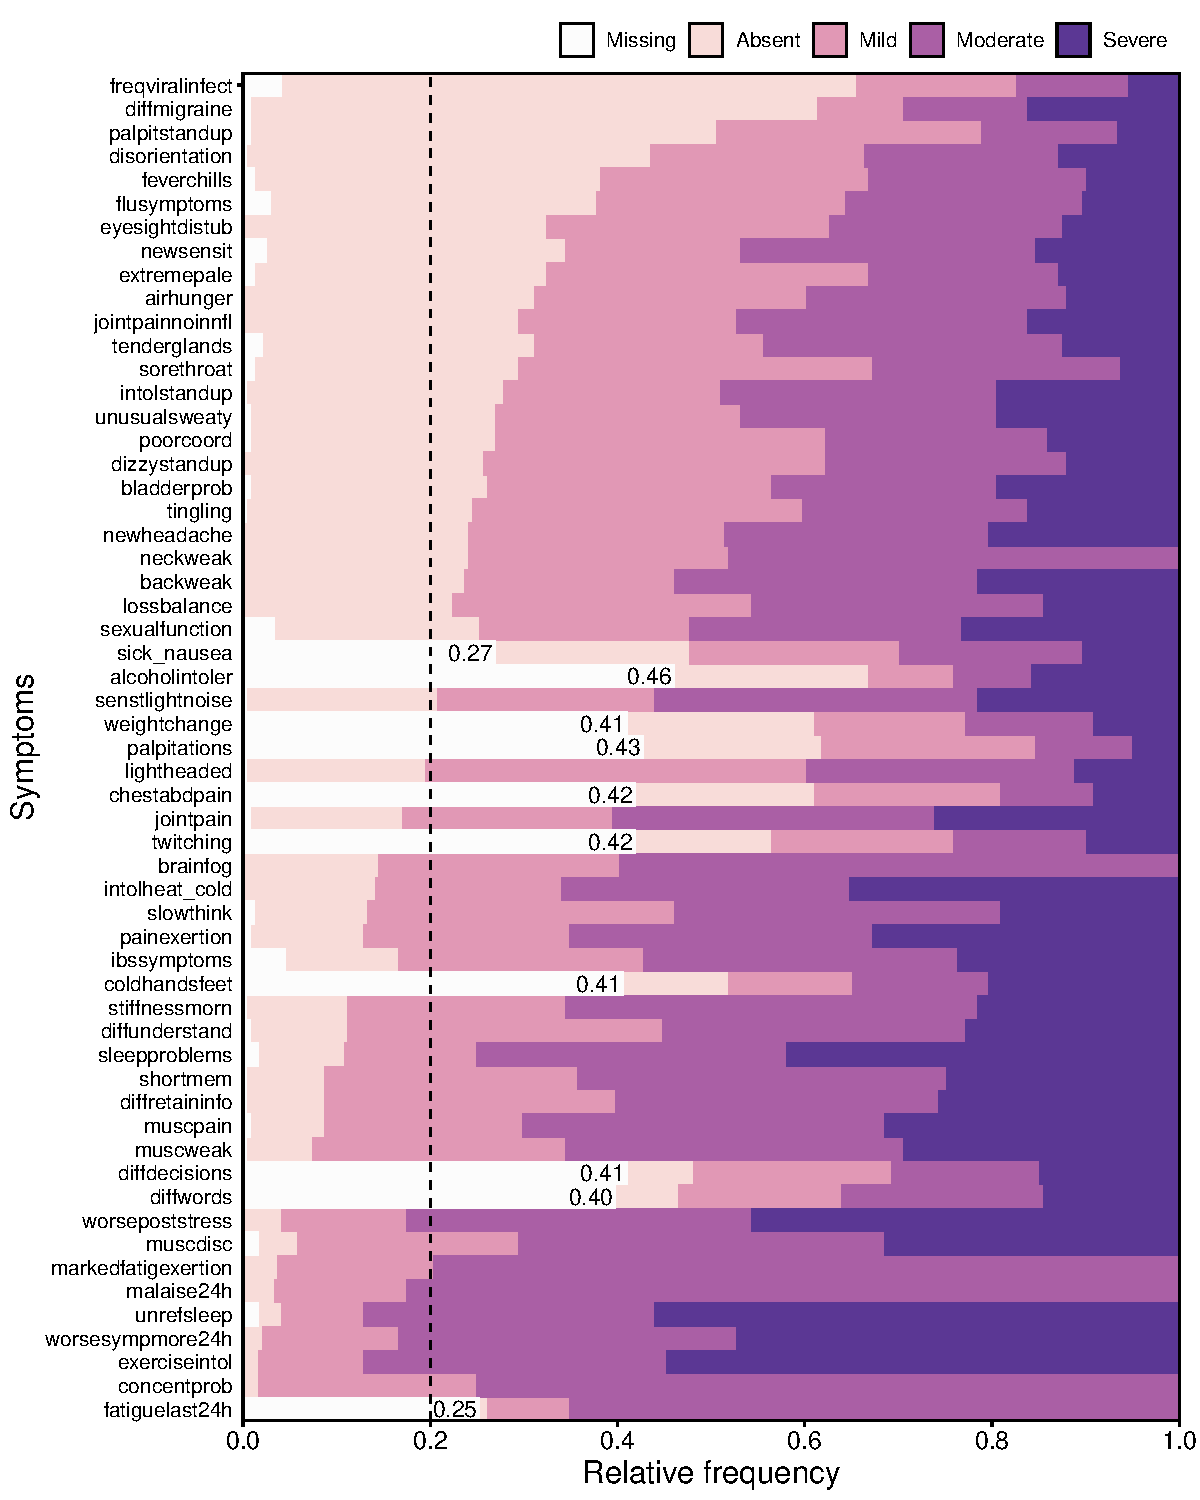
\includegraphics[width=0.95\textwidth]{chapter/2024-sym-domains/figures/figa1-ordinal-symptom-proportion-by-absent.pdf}
%     \caption[Relative frequency of ordinal degrees of severity on each one of the original 57 symptoms available across the population of ME/CFS patients]{Relative frequency of ordinal degrees of severity on each one of the original 57 symptoms available across the population of ME/CFS patients ($n = 241$). Symptoms are ordered by decreasing level of severity and relative proportion. Vertical dashed line at the 0.2 mark designates the missing values cutoff. Symptoms with a proportion of unreported (missing) severity across all individuals higher than that value were identified (relative proportions that surpass the cutoff are indicated in the missing columns) and removed from the analysis. A more detailed description of each symptom can be found elsewhere (Supplementary Table~\ref{appendix:taba2-sym-description}).}
%     \label{appendix:figa1-ordinal-symptom-proportion-by-absent}
% \end{figure}
% % Supplementary Figure 1
% % Supplementary Figure~\ref{appendix:figa1-quantitative-serology}


\begin{figure}[h]
    \centering
    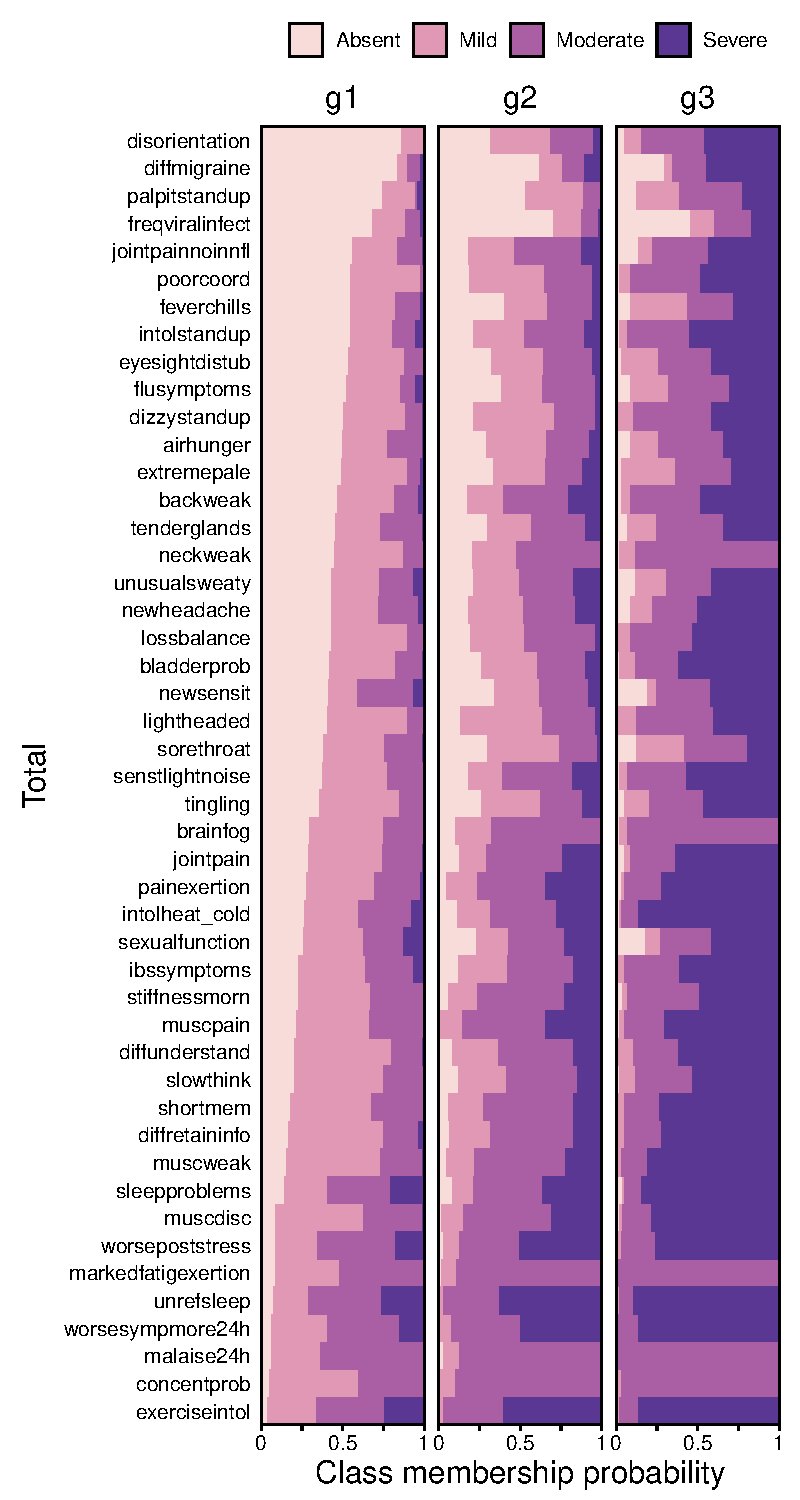
\includegraphics[height=0.7\paperheight]{chapter/2024-sym-domains/figures/figa2-lca-response-probabilities-bic-total-absent.pdf}
    \caption[Latent class analysis estimated class membership probabilities of symptom severities on different BIC-based subgroups, when profiling ME/CFS patients with the totality of available symptoms]{Latent class analysis estimated class membership probabilities of symptom severities on different BIC-based subgroups (latent classes), when profiling ME/CFS patients with the totality of available symptoms. Subgroups were ordered by increasing severity in the response probabilities of symptoms. A more detailed description of each symptom can be found elsewhere (Supplementary Table~\ref{appendix:taba2-sym-description}).}
    \label{appendix:figa2-lca-response-probabilities-bic-total-absent}
\end{figure}
% Supplementary Figure 2
% Supplementary Figure~\ref{appendix:figa2-lca-response-probabilities-bic-total-absent}


\begin{figure}[h]
    \centering
    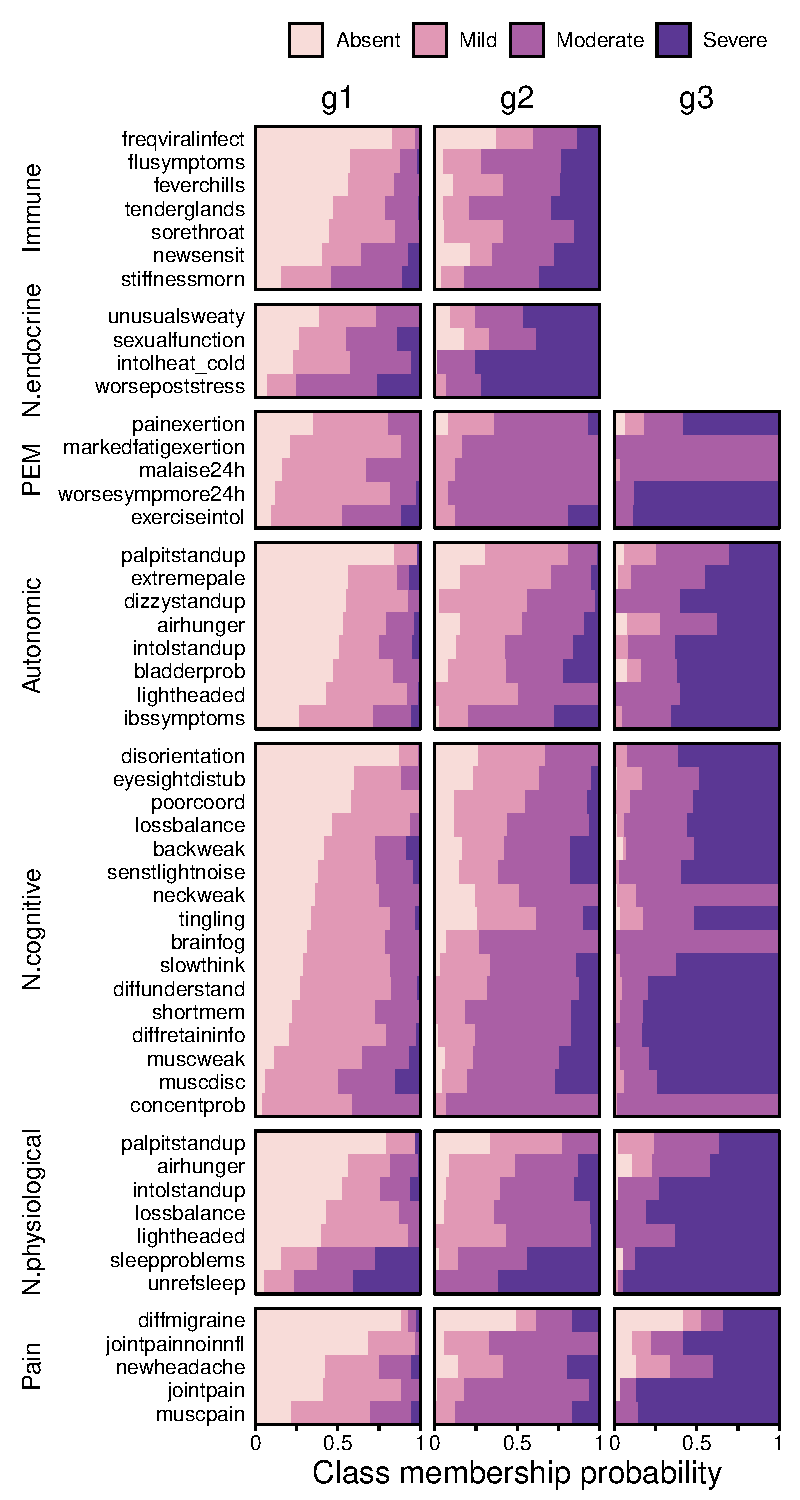
\includegraphics[height=0.7\paperheight]{chapter/2024-sym-domains/figures/figa3-lca-response-probabilities-bic-absent.pdf}
    \caption[Latent class analysis estimated class membership probabilities of symptom severities on different BIC-based subgroups, across the different domains]{Latent class analysis estimated class membership probabilities of symptom severities on different BIC-based subgroups (latent classes), across the different domains, autonomic, immunological, neurocognitive, neuroendocrine, neurophysiological, pain, and post-exertional malaise (PEM). For each domain, subgroups were ordered by increasing severity in the response probabilities of symptoms that make up each domain. A more detailed description of each symptom can be found elsewhere (Supplementary Table~\ref{appendix:taba2-sym-description}).}
    \label{appendix:figa3-lca-response-probabilities-bic-absent}
\end{figure}
% Supplementary Figure 3
% Supplementary Figure~\ref{appendix:figa3-lca-response-probabilities-bic-absent}